% ============================================================================
% MÓDULO 3 — CAPÍTULO 9
% Geossistemas, Ecodinâmica e Análise Empírica da Fragilidade Ambiental (Semana 9)
% ============================================================================

\chapter{Geossistemas, Ecodinâmica e Análise Empírica da Fragilidade Ambiental}
\label{cap:geossistemas_fragilidade}

\noindent\tagEmenta\ \tagPratica

\begin{capObjetivos}
Ao concluir este capítulo (Semana 9 do Plano CHF662), você será capaz de:
\begin{enumerate}[leftmargin=1.6em, itemsep=2pt]
  \item Explicar os princípios da \textbf{Teoria Geral dos Sistemas} (Bertalanffy, 2010) aplicados à paisagem, distinguindo totalidade, fluxos de matéria/energia, homeostase e propriedades emergentes.
  \item Classificar unidades espaciais segundo a \textbf{taxonomia da paisagem} de Bertrand (2004) (zona, domínio, região natural, geossistema, geofácies e geótopo) e aplicar a \textbf{compartimentação geoambiental} (Rodriguez; Silva; Cavalcanti, 2017) ao planejamento.
  \item Diagnosticar o estado dinâmico de unidades territoriais pela \textbf{Ecodinâmica de Tricart (1977)}, avaliando o balanço entre \textbf{morfogênese} e \textbf{pedogênese} em meios estáveis, intergrades e fortemente instáveis.
  \item Aplicar integralmente a \textbf{Análise Empírica da Fragilidade dos Ambientes Naturais e Antropizados} de \textbf{Ross (1994)}, atribuindo as cinco classes hierárquicas (1 a 5) para Relevo/Declividade, Solos, Clima/Pluviosidade e Uso da Terra/Cobertura Vegetal, além de calcular e interpretar os códigos da \textbf{Fragilidade Potencial ($FP$)} e da \textbf{Fragilidade Emergente ($FE$)}.
\end{enumerate}
\end{capObjetivos}

\begin{capRevisao}
Antes de avançar, retome três fundamentos consolidados nos capítulos anteriores:
\begin{itemize}[leftmargin=1.5em, itemsep=2pt]
  \item \textbf{Sistemas ambientais abertos e escalas (Cap. 6):} toda unidade da paisagem troca energia e matéria com o entorno e possui processos próprios em cada escala espacial e temporal; conclusões de detalhe não podem ser extrapoladas linearmente sem ajuste escalar.
  \item \textbf{Bacias hidrográficas e morfopedologia (Caps. 7 e 8):} a bacia fornece o recorte espacial funcional da drenagem, enquanto a vertente revela a interdependência entre declividade ($S\%$), classe de solo (topossequência) e escoamento superficial.
  \item \textbf{Classes de declividade de Ross (Cap. 8):} os cinco patamares de inclinação do terreno ($<6\%$, $6\text{--}12\%$, $12\text{--}20\%$, $20\text{--}30\%$ e $>30\%$) já dominados no Capítulo 8 constituem a primeira variável-chave da matriz de fragilidade ambiental estudada agora.
\end{itemize}
\end{capRevisao}

\etapa{3}{Explicação Teórica: Sistemas, Geossistemas, Ecodinâmica e Fragilidade Ambiental (Ross, 1994)}

\begin{boxSimbolo}[Vocabulário Técnico e Símbolos do Capítulo 9]
A análise integrada da paisagem apoia-se em conceitos sistêmicos e em uma notação específica de fragilidade. Um \textbf{sistema (Bertalanffy, 2010)} corresponde a um conjunto de elementos interdependentes em interação dinâmica, organizado como totalidade funcional capaz de receber entradas (\textit{inputs}), processá-las e emitir saídas (\textit{outputs}). Na escala geográfica, o \textbf{geossistema (Bertrand, 2004)} designa uma unidade espacial homogênea resultante da combinação dinâmica entre potencial ecológico (clima, relevo, hidrologia), exploração biológica (vegetação, solo, fauna) e ação antrópica, subdividindo-se em \textbf{geofácies}, setor fisionomicamente homogêneo (como uma encosta de Caatinga conservada), e em \textbf{geótopo}, a menor unidade espacial (como uma ravina ou afloramento rochoso).

Para diagnosticar o estado dinâmico dessas unidades, a \textbf{Ecodinâmica (Tricart, 1977)} avalia o balanço entre processos de remoção e erosão (\textbf{morfogênese}) e processos de formação de solo (\textbf{pedogênese}). Operacionalmente, a \textbf{Fragilidade Potencial ($FP$)} expressa a suscetibilidade natural intrínseca do ambiente à degradação e à erosão, determinada pelos fatores físicos ($D_R$: Relevo/Declividade; $D_S$: Solos; $D_C$: Clima/Pluviosidade), independentemente da vegetação atual, ao passo que a \textbf{Fragilidade Emergente ($FE$)} traduz a fragilidade real atual, obtida pelo cruzamento de $FP$ com o grau de proteção conferido pelo Uso da Terra e Cobertura Vegetal ($D_U$). Essa informação é sintetizada no \textbf{Código Numérico de Ross}, uma notação posicional formada pelos dígitos das classes de $1$ a $5$, com três dígitos para $FP$ ($D_R D_S D_C$) e quatro dígitos para $FE$ ($D_R D_S D_C D_U$), acompanhada da respectiva classe síntese ($1$ a $5$).
\end{boxSimbolo}

\section{Teoria Geral dos Sistemas (Bertalanffy, 2010) na Análise Ambiental}

Até meados do século XX, grande parte das ciências naturais operava de modo analítico-reducionista, isolando o solo da rocha, a vegetação do clima e o rio das encostas. Ao formular a \textbf{Teoria Geral dos Sistemas (TGS)}, o biólogo \textbf{Ludwig von Bertalanffy (2010)} demonstrou que sistemas complexos não podem ser compreendidos pela simples soma de suas partes isoladas, pois suas propriedades essenciais emergem justamente das \textbf{relações e interações} entre os componentes.

Na Análise Ambiental, a adoção da TGS traduz-se em quatro princípios operacionais articulados. Pelo princípio da \textbf{totalidade e interdependência}, alterar qualquer componente, como remover a cobertura vegetal de uma encosta, modifica imediatamente a infiltração, o escoamento superficial, a temperatura do solo, a erosão e o regime de sedimentos do rio a jusante. Paisagens e bacias hidrográficas operam como \textbf{sistemas abertos e de fluxos contínuos}, recebendo energia solar e precipitação (\textit{inputs}), transformando esses fluxos internamente e exportando água, sedimentos, calor e nutrientes (\textit{outputs}). Sob condições conservadas, esses sistemas mantêm um \textbf{equilíbrio dinâmico (homeostase)} próximo a um estado estacionário graças a mecanismos de autorregulação (\textit{feedback} negativo), mas quando perturbações antrópicas ultrapassam a capacidade de suporte, instala-se a retroalimentação positiva e a degradação acelera-se. Dessa interação conjunta nasce a \textbf{propriedade emergente}, razão pela qual a \textbf{fragilidade ambiental} pertence à combinação simultânea entre os fatores físicos e o uso humano da terra, e nunca a um elemento isolado.

\section{Geossistema, Taxonomia da Paisagem e Compartimentação Geoambiental}

Inspirado na TGS e na escola russo-soviética (Sochava), o geógrafo francês \textbf{Georges Bertrand (2004)} propôs o conceito de \textbf{geossistema} como unidade fundamental para a Geografia Física integrada. Enquanto o ecossistema privilegia as relações tróficas biológicas sem escala espacial rígida, o \textbf{geossistema constitui uma unidade territorial concreta}, situada em uma escala definida (da ordem de alguns quilômetros quadrados a centenas de quilômetros quadrados), onde interagem três conjuntos de forças. O \textbf{Potencial Ecológico} fornece a base abiótica formada por geologia, geomorfologia, clima e hidrologia; a \textbf{Exploração Biológica} reúne vegetação, solos e fauna que colonizam e protegem essa base; e a \textbf{Ação Antrópica} expressa a organização socioeconômica, o uso da terra e as intervenções técnicas que transformam ou conservam o conjunto.

Para evitar a confusão entre escalas regionais e locais (a falácia de escala vista no Cap. 6), Bertrand (2004) estruturou uma \textbf{taxonomia hierárquica da paisagem} em seis níveis, organizados das unidades superiores (zonais/estruturais) às unidades inferiores (dinâmicas/locais), conforme sintetiza a Tabela~\ref{tab:taxonomia_bertrand}.

\begin{table}[H]
\centering
\caption{Taxonomia hierárquica da paisagem segundo Bertrand (2004) e articulação escalar (Rodriguez; Silva; Cavalcanti, 2017).}
\label{tab:taxonomia_bertrand}
\renewcommand{\arraystretch}{1.18}
\small
\begin{tabularx}{\textwidth}{@{}p{2.3cm} p{2.2cm} p{2.3cm} p{3.1cm} >{\raggedright\arraybackslash}X@{}}
  \toprule
  \rowcolor{uefsNavy}
  \textcolor{white}{\bfseries Unidade} & \textcolor{white}{\bfseries Ordem (Escala G)} & \textcolor{white}{\bfseries Escala Cartográfica} & \textcolor{white}{\bfseries Critério Definidor Principal} & \textcolor{white}{\bfseries Exemplo no Brasil / Semiárido} \\
  \midrule
  \multicolumn{5}{@{}l}{\cellcolor{bgGold}\textbf{\color{uefsNavy}Unidades Superiores (condicionamento climático-estrutural)}} \\
  1. Zona & $G\text{I}$ ($>10^7\text{ km}^2$) & $< 1:10.000.000$ & Grandes faixas climáticas planetárias & Zona Intertropical. \\
  \rowcolor{bgGray}
  2. Domínio & $G\text{II}$ ($10^6\text{ km}^2$) & $1:5.000.000$ & Macroestrutura climática, relevo e bioma & Domínio das Caatingas / Depressões Sertanejas. \\
  3. Região Natural & $G\text{III}\text{--}G\text{IV}$ & $1:1.000.000$ & Compartimento geomorfológico e clima regional & Piemonte da Diamantina / Bacia do Rio Jacuípe. \\
  \midrule
  \multicolumn{5}{@{}l}{\cellcolor{bgTeal}\textbf{\color{uefsNavy}Unidades Inferiores (dinâmica integrada e diagnóstico aplicado)}} \\
  4. Geossistema & $G\text{V}$ ($10^1\text{--}10^2\text{ km}^2$) & $1:50.000$ a $1:100.000$ & Combinação potencial ecológico + exploração biológica + antrópica & Geossistema da Serra de São José (Feira de Santana/BA) ou Sub-bacia do Vaza-Barris. \\
  \rowcolor{bgGray}
  5. Geofácies & $G\text{VI}$ ($10^{-1}\text{--}10^0\text{ km}^2$) & $1:10.000$ a $1:25.000$ & Fisionomia homogênea de relevo, solo e cobertura vegetal & Meia encosta com Caatinga arbustiva raleada sobre Neossolo Litólico. \\
  6. Geótopo & $G\text{VII}$ ($<10^{-2}\text{ km}^2$) & $> 1:5.000$ & Microunidade de detalhe extremo e microclima próprio & Parede de voçoroca ativa, lajedo ou talude rodoviário. \\
  \bottomrule
\end{tabularx}
\end{table}

Na prática da Análise Ambiental no Brasil, \textbf{Rodriguez, Silva e Cavalcanti (2017)} avançam da taxonomia descritiva para a \textbf{compartimentação geoambiental}. Compartimentar significa delimitar sobre o mapa \textbf{unidades geoambientais} relativamente homogêneas quanto à sua gênese, morfologia, pedologia, drenagem e uso atual, de modo que cada compartimento receba diretrizes próprias de conservação, recuperação ou uso produtivo no ordenamento territorial.

\section{Ecodinâmica de Tricart (1977): Balanço Morfogênese vs. Pedogênese}

Enquanto Bertrand organizou a paisagem em níveis espaciais, o geomorfólogo francês \textbf{Jean Tricart (1977)} propôs classificar os ambientes segundo o seu \textbf{grau de estabilidade dinâmica}. O critério central da \textbf{Ecodinâmica} reside no balanço energético entre dois processos opostos que atuam simultaneamente em qualquer vertente. De um lado, a \textbf{pedogênese} reúne os processos físicos, químicos e biológicos que promovem o intemperismo das rochas, a infiltração da água e a formação ou espessamento dos horizontes do solo; de outro, a \textbf{morfogênese} agrupa os processos erosivos, gravitacionais e de escoamento que removem partículas da superfície, rebaixam o manto de alteração e modelam o relevo.

A partir dessa competição contínua, Tricart (1977) estabelece \textbf{três grandes tipos de meios ecodinâmicos}, detalhados na Tabela~\ref{tab:ecodinamica_tricart}. Nos \textbf{meios estáveis}, a cobertura vegetal densa e o relevo suave permitem que a infiltração domine o balanço hídrico, de modo que a pedogênese supera amplamente a morfogênese ($P \gg M$). Nos \textbf{meios intergrades (ou de transição)}, instala-se um equilíbrio dinâmico tenso ($P \approx M$), no qual a infiltração e o escoamento superficial competem continuamente, tornando o ambiente suscetível a desequilíbrios rápidos caso o manejo seja inadequado. Já nos \textbf{meios fortemente instáveis}, a combinação de declividades acentuadas, solos rasos ou expostos e chuvas concentradas faz a morfogênese predominar francamente sobre a pedogênese ($M \gg P$), disparando erosão linear e movimentos de massa.

\begin{table}[H]
\centering
\caption{Classificação ecodinâmica dos ambientes segundo Tricart (1977) e implicações para o planejamento.}
\label{tab:ecodinamica_tricart}
\renewcommand{\arraystretch}{1.20}
\small
\begin{tabularx}{\textwidth}{@{}p{2.6cm} p{2.9cm} p{3.0cm} >{\raggedright\arraybackslash}X@{}}
  \toprule
  \rowcolor{uefsNavy}
  \textcolor{white}{\bfseries Meio Ecodinâmico} & \textcolor{white}{\bfseries Balanço Morfogênese vs. Pedogênese} & \textcolor{white}{\bfseries Características Típicas} & \textcolor{white}{\bfseries Manejo e Fragilidade} \\
  \midrule
  \textbf{Meios Estáveis} & \textbf{Pedogênese supera amplamente a morfogênese} ($P \gg M$) & Cobertura vegetal densa e contínua; relevo suave ou plano; solos profundos (Latossolos); dissecação incipiente; ausência de erosão acelerada. & Baixa fragilidade natural. Suportam uso agrícola tecnificado com práticas conservacionistas preventivas; o desmatamento pode romper a estabilidade. \\
  \rowcolor{bgGray}
  \textbf{Meios Intergrades (de Transição)} & \textbf{Equilíbrio dinâmico tenso} ($P \approx M$) & Interferência permanente entre infiltração/pedogênese e escoamento/morfogênese; vertentes moderadamente inclinadas ou áreas com vegetação rala/alterada. & Suscetíveis a desequilíbrios rápidos se manejados sem critério. Exigem práticas rigorosas de conservação do solo (curvas de nível, cobertura morta, manejo de pastagem). \\
  \textbf{Meios Fortemente Instáveis} & \textbf{Morfogênese predomina francamente} ($M \gg P$) & Declividades elevadas ($>20\text{--}30\%$); solos rasos (Neossolos Litólicos) ou expostos; clima agressivo/torrencial; ocorrência de ravinas, voçorocas ou movimentos de massa. & Máxima restrição ao uso intensivo. Prioridade absoluta para preservação, bioengenharia de solos, controle de drenagem e recuperação ambiental. \\
  \bottomrule
\end{tabularx}
\end{table}

A Figura~\ref{fig:ecodinamica_ross} ilustra a ponte metodológica entre essa leitura qualitativa dos meios ecodinâmicos de Tricart ((a)) e sua operacionalização cartográfica na Matriz de Fragilidade Emergente de Ross ((b)).

\begin{figure}[H]
  \centering
  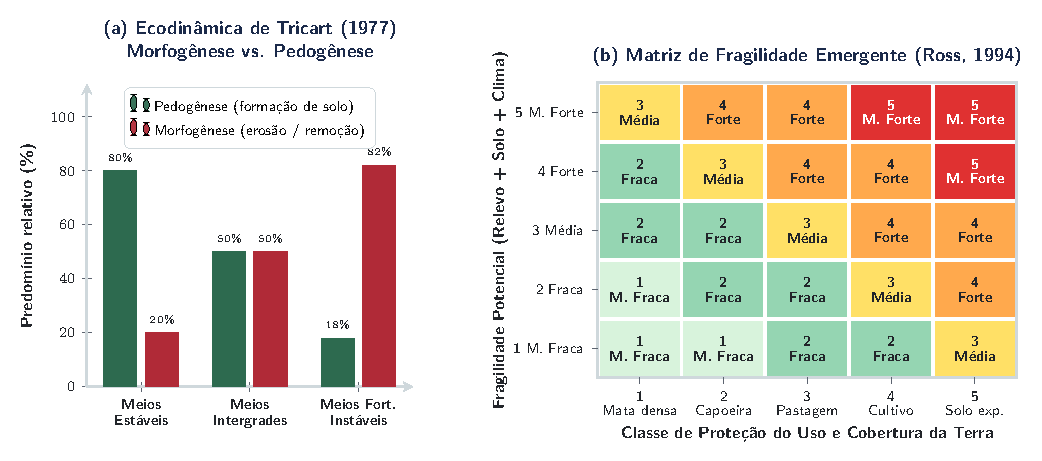
\includegraphics[width=0.95\textwidth]{figures/fig07_ecodinamica_ross_matriz.pdf}
  \caption{Integração metodológica entre a Ecodinâmica de Tricart (1977), expressa pelo balanço relativo entre pedogênese e morfogênese nos três tipos de meios ((a)), e a Matriz de Fragilidade Emergente de Ross (1994), obtida pelo cruzamento da Fragilidade Potencial com o grau de proteção do Uso da Terra ((b)).}
  \label{fig:ecodinamica_ross}
\end{figure}

\section{Análise Empírica da Fragilidade Ambiental (Ross, 1994)}

Na década de 1990, o geógrafo brasileiro \textbf{Jurandyr Luciano Sanches Ross (1994)} operacionalizou os princípios dos Geossistemas e da Ecodinâmica de Tricart em uma metodologia cartográfica e quantitativa padronizada: a \textbf{Análise Empírica da Fragilidade dos Ambientes Naturais e Antropizados}. Para manter a coerência com Tricart, Ross substituiu a expressão ``meios estáveis/instáveis'' por \textbf{Unidades Ecodinâmicas Estáveis} e \textbf{Unidades Ecodinâmicas de Instabilidade Potencial ou Emergente}, classificadas em \textbf{cinco graus hierárquicos}:
\[
  1 = \text{Muito Fraca} \quad;\quad 2 = \text{Fraca} \quad;\quad 3 = \text{Média} \quad;\quad 4 = \text{Forte} \quad;\quad 5 = \text{Muito Forte}.
\]

\begin{boxConceito}[Distinção Fundamental: Fragilidade Potencial vs. Fragilidade Emergente]
A \textbf{Fragilidade Potencial ($FP$)} expressa a suscetibilidade \emph{natural e intrínseca} do terreno antes de considerar a ação humana ou a vegetação atual, combinando exclusivamente os fatores do meio físico: \textbf{Relevo/Declividade ($D_R$)}, \textbf{Solos ($D_S$)} e \textbf{Clima/Pluviosidade ($D_C$)}. Ela responde à pergunta: \emph{``Quão vulnerável este terreno seria se perdesse sua cobertura vegetal?''} Já a \textbf{Fragilidade Emergente ($FE$)} traduz a suscetibilidade \emph{real e atual} do ambiente, resultando do cruzamento entre a \textbf{Fragilidade Potencial ($FP$)} e o grau de proteção oferecido pelo \textbf{Uso da Terra / Cobertura Vegetal ($D_U$)}, respondendo à questão: \emph{``Qual é o risco efetivo de degradação hoje, considerando o uso e a vegetação existentes?''}
\end{boxConceito}

\subsection{Tabelas Completas das Cinco Classes Hierárquicas de Ross (1994)}

As Tabelas~\ref{tab:ross_relevo_solos} e~\ref{tab:ross_clima_uso} apresentam os critérios completos das quatro variáveis básicas utilizadas na metodologia de Ross (1994). Em estudos de detalhe (microbacias e municípios, escalas de $1:10.000$ a $1:50.000$), adota-se a \textbf{declividade ($S\%$)} como indicador do relevo; em estudos regionais (escalas menores que $1:100.000$), utilizam-se os índices de dissecação do relevo (entalhamento de vales e dimensão interfluvial).

\begin{table}[H]
\centering
\caption{Classes hierárquicas de fragilidade para Relevo/Declividade ($D_R$) e Solos ($D_S$) segundo Ross (1994).}
\label{tab:ross_relevo_solos}
\renewcommand{\arraystretch}{1.18}
\small
\begin{tabularx}{\textwidth}{@{}p{1.9cm} p{2.9cm} p{3.5cm} >{\raggedright\arraybackslash}X@{}}
  \toprule
  \rowcolor{uefsNavy}
  \textcolor{white}{\bfseries Classe / Grau} & \textcolor{white}{\bfseries Declividade ($D_R$)} & \textcolor{white}{\bfseries Dissecação Regional ($D_R$)} & \textcolor{white}{\bfseries Classes de Solos / Erodibilidade ($D_S$)} \\
  \midrule
  \textbf{1, Muito Fraca} & $< 6\%$ & Muito fraca (vales muito rasos, interflúvios amplos) & Latossolos Roxos e Vermelho-Escuros de textura argilosa (muito profundos e bem estruturados). \\
  \rowcolor{bgGray}
  \textbf{2, Fraca} & $6\text{ a } 12\%$ & Fraca (entalhamento e densidade baixos) & Latossolos Vermelho-Amarelos de textura média/argilosa; Nitossolos profundos. \\
  \textbf{3, Média} & $12\text{ a } 20\%$ & Média (vertentes moderadamente dissecadas) & Latossolos Amarelos/Vermelho-Amarelos arenosos; Argissolos profundos; Cambissolos profundos. \\
  \rowcolor{bgGray}
  \textbf{4, Forte} & $20\text{ a } 30\%$ & Forte (vales entalhados e interflúvios estreitos) & Argissolos com mudança textural abrupta; Planossolos (comum no Semiárido); Cambissolos rasos/siltosos. \\
  \textbf{5, Muito Forte} & $> 30\%$ & Muito forte (escarpas, vales muito profundos) & Neossolos Litólicos (solos rasos sobre rocha), Neossolos Quartzarênicos (areias quartzosas), Gleissolos e Organossolos em áreas instáveis. \\
  \bottomrule
\end{tabularx}
\end{table}

Definidos os graus de vulnerabilidade intrínseca do relevo e dos solos na Tabela~\ref{tab:ross_relevo_solos}, o analista incorpora a agressividade climática (erosividade das chuvas) e o efeito protetor ou degradante da cobertura vegetal por meio dos critérios da Tabela~\ref{tab:ross_clima_uso}.

\begin{table}[H]
\centering
\caption{Classes hierárquicas de fragilidade para Clima/Pluviosidade ($D_C$) e Uso da Terra / Cobertura Vegetal ($D_U$) segundo Ross (1994).}
\label{tab:ross_clima_uso}
\renewcommand{\arraystretch}{1.18}
\small
\begin{tabularx}{\textwidth}{@{}p{1.9cm} p{5.5cm} >{\raggedright\arraybackslash}X@{}}
  \toprule
  \rowcolor{uefsNavy}
  \textcolor{white}{\bfseries Classe / Grau} & \textcolor{white}{\bfseries Clima / Pluviosidade ($D_C$, Erosividade)} & \textcolor{white}{\bfseries Uso da Terra / Cobertura Vegetal ($D_U$, Grau de Proteção)} \\
  \midrule
  \textbf{1, Muito Fraca} & Pluviosidade regular ao longo do ano, baixa intensidade horária, sem concentração extrema. & \textbf{Proteção Muito Alta:} florestas naturais primárias, matas ciliares densas e Caatinga arbórea fechada. \\
  \rowcolor{bgGray}
  \textbf{2, Fraca} & Precipitação moderada ($1.000\text{--}1.300\text{ mm/ano}$) com estação seca curta e chuvas pouco torrenciais. & \textbf{Proteção Alta:} florestas secundárias avançadas (capoeirões), Caatinga arbustivo-arbórea densa, silvicultura bem manejada. \\
  \textbf{3, Média} & Estação seca definida ($3\text{--}6$ meses) e chuvas concentradas no verão/outono com eventos erosivos moderados. & \textbf{Proteção Média:} pastagens bem manejadas com boa cobertura, sistemas agroflorestais (SAFs), culturas perenes (café, cacau em cabruca). \\
  \rowcolor{bgGray}
  \textbf{4, Forte} & Forte concentração pluviométrica sazonal (ou totais $>2.000\text{ mm/ano}$ com aguaceiros intensos). & \textbf{Proteção Baixa:} culturas temporárias de ciclo curto (milho, feijão, mandioca), pastagens degradadas/raleadas e áreas de queimada antiga. \\
  \textbf{5, Muito Forte} & Chuvas altamente concentradas e torrenciais (típico do Semiárido com aguaceiros sobre solo seco, ou áreas de extrema erosividade). & \textbf{Proteção Muito Baixa / Nula:} solo exposto, áreas terraplanadas, mineração, queimada recente, área urbana sem drenagem. \\
  \bottomrule
\end{tabularx}
\end{table}

\subsection{Cálculo e Leitura do Código Numérico de Ross ($FP$ e $FE$)}

Na metodologia de Ross (1994), cada unidade geoambiental recebe um \textbf{código numérico posicional} que preserva a memória individual de cada variável, impedindo que a causa do problema desapareça na média. O \textbf{Código da Fragilidade Potencial ($FP$)} é formado por \textbf{três dígitos} na ordem fixa $\mathbf{D_R\,D_S\,D_C}$ (Relevo, Solos e Clima), enquanto o \textbf{Código da Fragilidade Emergente ($FE$)} acrescenta o fator antrópico e passa a contar com \textbf{quatro dígitos} na ordem fixa $\mathbf{D_R\,D_S\,D_C\,D_U}$ (Relevo, Solos, Clima e Uso da Terra).

\begin{boxFormula}[Cálculo e Leitura da Fragilidade Potencial ($FP$) e Fragilidade Emergente ($FE$)]
\textbf{Passo 1, Atribuição dos dígitos ($1$ a $5$):} enquadre o terreno nas Tabelas~\ref{tab:ross_relevo_solos} e~\ref{tab:ross_clima_uso}, obtendo $D_R$, $D_S$, $D_C$ e $D_U$.

\textbf{Passo 2, Montagem dos códigos posicionais:}
\[
  \text{Código } FP = D_R\,D_S\,D_C \qquad\text{e}\qquad \text{Código } FE = D_R\,D_S\,D_C\,D_U.
\]

\textbf{Passo 3, Determinação da Classe Síntese de $FP$ (1 a 5):} calcula-se a média aritmética das três variáveis físicas e arredonda-se para o inteiro mais próximo de $1$ a $5$ (em empates de $0{,}5$, adota-se o valor mais conservador ou o peso dominante do relevo $D_R$):
\[
  I_{FP} = \frac{D_R + D_S + D_C}{3} \quad \xrightarrow{\text{arredondamento}} \quad \text{Classe } FP \in \{1, 2, 3, 4, 5\}.
\]

\textbf{Passo 4, Determinação da Classe Síntese de $FE$ (1 a 5) na Matriz de Fragilidade Emergente:} cruza-se a \textbf{Classe $FP$} (linha) com o dígito do \textbf{Uso da Terra $D_U$} (coluna) na adaptação didático-operacional da matriz de Ross (1994) e Spörl e Ross (2004) apresentada abaixo (Figura~\ref{fig:ecodinamica_ross}, (b)). Nos casos em que $(FP + D_U)/2$ resulta em fração $0{,}5$, a matriz pondera o efeito protetor da cobertura vegetal densa ($D_U \le 2$, arredondando para baixo) em contraste com o agravamento imposto por usos antrópicos expostos ($D_U \ge 3$, arredondando para cima):

\begin{center}
\renewcommand{\arraystretch}{1.12}
\footnotesize
\begin{tabular}{@{}l|ccccc@{}}
  \toprule
  \textbf{Fragilidade Potencial ($FP$)} $\backslash$ \textbf{Uso ($D_U$)} & \textbf{1 (M. Alta Prot.)} & \textbf{2 (Alta)} & \textbf{3 (Média)} & \textbf{4 (Baixa)} & \textbf{5 (Nula)} \\
  \midrule
  \textbf{1, Muito Fraca} & 1 (M. Fraca) & 1 (M. Fraca) & 2 (Fraca) & 2 (Fraca) & 3 (Média) \\
  \textbf{2, Fraca} & 1 (M. Fraca) & 2 (Fraca) & 2 (Fraca) & 3 (Média) & 4 (Forte) \\
  \textbf{3, Média} & 2 (Fraca) & 2 (Fraca) & 3 (Média) & 4 (Forte) & 4 (Forte) \\
  \textbf{4, Forte} & 2 (Fraca) & 3 (Média) & 4 (Forte) & 4 (Forte) & 5 (M. Forte) \\
  \textbf{5, Muito Forte} & 3 (Média) & 4 (Forte) & 4 (Forte) & 5 (M. Forte) & 5 (M. Forte) \\
  \bottomrule
\end{tabular}
\end{center}
\vspace{2pt}
{\footnotesize\emph{Nota:} na célula $(FP=5, D_U=1)$, a proteção florestal primária reduz a fragilidade emergente para \textbf{3, Média}.}

\textbf{Exemplo numérico completo:} considere uma encosta com declividade $S = 22\%$ ($D_R = 4$), Argissolo profundo ($D_S = 3$), clima semiárido com chuvas torrenciais concentradas ($D_C = 4$) e pastagem degradada ($D_U = 4$). O \textbf{Código $FP$} resulta em $\mathbf{434}$, cuja média $I_{FP} = (4 + 3 + 4)/3 = 11/3 \approx 3{,}67$ conduz à \textbf{Classe $FP = 4$ (Forte)}. Ao incorporar o uso atual, obtém-se o \textbf{Código $FE$} igual a $\mathbf{4344}$, e o cruzamento de $FP = 4$ com $D_U = 4$ na matriz acima confirma a \textbf{Classe $FE = 4$ (Forte)}. Na leitura técnica do código $4344$, o primeiro dígito ($4$) alerta que a declividade ($20\text{--}30\%$) é o principal motor físico da instabilidade, o terceiro dígito ($4$) indica forte erosividade climática, e o quarto dígito ($4$) revela que a pastagem degradada deixa o solo desprotegido, mantendo o risco real elevado (Classe 4).
\end{boxFormula}

\etapa{4}{Estudos de Caso e Exemplos Resolvidos}

\begin{boxExemplo}{9.1}{Enquadramento na Taxonomia da Paisagem de Bertrand (Nível Básico)}
\passoEnunciado{Uma equipe de Análise Ambiental da UEFS está diagnosticando processos erosivos em uma propriedade rural próxima a Feira de Santana (BA). Durante o trabalho, os estudantes precisam situar espacialmente quatro recortes: (I) o Domínio das Caatingas; (II) a sub-bacia do Rio Jacuípe (escala $1:100.000$); (III) uma vertente homogênea de pastagem sobre Argissolo ($1:15.000$); e (IV) uma voçoroca ativa com $40\,\text{m}$ de comprimento ($1:1.000$).}
\passoDados{Quatro recortes espaciais com escalas variando de continental/regional ($G\text{II}$) até o detalhe local ($G\text{VII}$).}
\passoPedido{Enquadrar corretamente cada recorte (I a IV) nas unidades taxonômicas de Bertrand (2004).}
\passoMetodo{Aplicação direta da Tabela~\ref{tab:taxonomia_bertrand} (unidades superiores e inferiores segundo ordem de grandeza e critério definidor).}
\passoContas{%
\begin{enumerate}[leftmargin=1.6em, itemsep=1.5pt]
  \item \textbf{Recorte I (Domínio das Caatingas):} escala regional/subcontinental ($G\text{II}$, $\sim 10^6\text{ km}^2$) definida por macroclima e bioma $\implies$ \textbf{Domínio}.
  \item \textbf{Recorte II (Sub-bacia em $1:100.000$):} unidade funcional concreta ($G\text{V}$, dezenas a centenas de $\text{km}^2$) que integra potencial ecológico, exploração biológica e ação antrópica $\implies$ \textbf{Geossistema}.
  \item \textbf{Recorte III (Vertente homogênea em $1:15.000$):} setor fisionomicamente uniforme dentro do geossistema ($G\text{VI}$) $\implies$ \textbf{Geofácies}.
  \item \textbf{Recorte IV (Voçoroca de $40\,\text{m}$ em $1:1.000$):} menor unidade espacial de detalhe extremo ($G\text{VII}$) $\implies$ \textbf{Geótopo}.
\end{enumerate}}
\passoResposta{I = Domínio; II = Geossistema; III = Geofácies; IV = Geótopo.}
\passoVerificacao{A sequência segue exatamente a ordem decrescente de grandeza espacial da taxonomia de Bertrand ($G\text{II} \to G\text{V} \to G\text{VI} \to G\text{VII}$), evitando misturar unidades regionais com feições pontuais de campo.}
\end{boxExemplo}

\begin{boxExemplo}{9.2}{Diagnóstico Ecodinâmico de Tricart em Três Setores de Sub-bacia (Nível Básico–Intermediário)}
\passoEnunciado{Ao percorrer uma sub-bacia do Piemonte da Chapada Diamantina, um geógrafo observou três compartimentos distintos: \textbf{Setor X}, chapada plana com vegetação arbórea conservada, Latossolo profundo e ausência de sulcos; \textbf{Setor Y}, rampa suave ($9\%$) com pastagem manejada, onde ocorrem infiltração moderada e leve escoamento laminar após chuvas fortes; \textbf{Setor Z}, encosta íngreme ($35\%$) desmatada, com Neossolo Litólico raso, ravinas profundas e blocos rolados.}
\passoDados{Setor X (plano, florestado, solo profundo); Setor Y ($S=9\%$, pastagem, erosão laminar leve); Setor Z ($S=35\%$, desmatado, solo raso, ravinas).}
\passoPedido{Classificar cada setor segundo a Ecodinâmica de Tricart (1977), explicando o balanço morfogênese vs. pedogênese.}
\passoMetodo{Comparação dos processos dominantes com os critérios da Tabela~\ref{tab:ecodinamica_tricart} e do (a) da Figura~\ref{fig:ecodinamica_ross}.}
\passoContas{%
\begin{enumerate}[leftmargin=1.6em, itemsep=1.5pt]
  \item \textbf{Setor X:} a cobertura arbórea e o relevo plano maximizam a infiltração e o intemperismo químico profundo, bloqueando a erosão superficial ($P \gg M$) $\implies$ \textbf{Meio Estável}.
  \item \textbf{Setor Y:} há competição equilibrada entre infiltração sob pastagem e remoção laminar nas chuvas intensas ($P \approx M$) $\implies$ \textbf{Meio Intergrade (de Transição)}.
  \item \textbf{Setor Z:} a alta declividade aliada à remoção da vegetação dispara erosão linear e perda acelerada de solo ($M \gg P$) $\implies$ \textbf{Meio Fortemente Instável}.
\end{enumerate}}
\passoResposta{Setor X = Meio Estável; Setor Y = Meio Intergrade; Setor Z = Meio Fortemente Instável.}
\passoVerificacao{O diagnóstico orienta diretamente a gestão: no Setor Z a prioridade é contenção erosiva e revegetação; no Setor Y, manejo conservacionista para impedir que o meio intergrade migre para a instabilidade forte.}
\end{boxExemplo}

\begin{boxExemplo}{9.3}{Cálculo Passo a Passo da Fragilidade Potencial e Emergente (Nível Intermediário)}
\passoEnunciado{Uma unidade geoambiental utilizada para estudo de planejamento municipal apresenta declividade média de $S = 15\%$, solo classificado como Argissolo profundo de textura média/argilosa, clima tropical semiárido com chuvas concentradas e torrenciais ($D_C = 4$) e uso atual por cultura temporária de mandioca em solo parcialmente descoberto.}
\passoDados{$S = 15\%$; Argissolo profundo; $D_C = 4$; uso por cultura temporária de ciclo curto.}
\passoPedido{Determinar os dígitos $D_R$, $D_S$, $D_C$ e $D_U$, montar os códigos numéricos de $FP$ e $FE$ e obter as classes síntese de Fragilidade Potencial e Emergente.}
\passoMetodo{Enquadramento pelas Tabelas~\ref{tab:ross_relevo_solos} e~\ref{tab:ross_clima_uso} e aplicação do roteiro de cálculo de Ross (1994).}
\passoContas{%
\begin{enumerate}[leftmargin=1.6em, itemsep=1.5pt]
  \item \textbf{Atribuição dos dígitos:}
  \begin{itemize}[leftmargin=1.4em, itemsep=1pt]
    \item Relevo ($S = 15\%$, faixa $12\text{--}20\%$): $D_R = 3$ (Média).
    \item Solos (Argissolo profundo): $D_S = 3$ (Média).
    \item Clima (fornecido): $D_C = 4$ (Forte).
    \item Uso da Terra (cultura temporária de ciclo curto): $D_U = 4$ (Proteção Baixa / Fragilidade Forte).
  \end{itemize}
  \item \textbf{Fragilidade Potencial ($FP$):} código posicional $\mathbf{334}$. Média física:
  \[
    I_{FP} = \frac{3 + 3 + 4}{3} = \frac{10}{3} \approx 3{,}33 \implies \text{Classe } FP = \mathbf{3\text{ (Média)}}.
  \]
  \item \textbf{Fragilidade Emergente ($FE$):} código posicional $\mathbf{3344}$. Cruzando $FP = 3$ com $D_U = 4$ na Matriz de Ross (Figura~\ref{fig:ecodinamica_ross}, (b)) $\implies$ \textbf{Classe $FE = 4$ (Forte)}.
\end{enumerate}}
\passoResposta{Código $FP = 334$ (Classe 3, Média); Código $FE = 3344$ (Classe 4, Forte).}
\passoVerificacao{Note o papel agravante do uso agrícola anual ($D_U = 4$): a unidade possui fragilidade natural média ($3$), mas o cultivo temporário com baixa proteção eleva a fragilidade real emergente para forte ($4$), exigindo plantio em nível e cobertura morta.}
\end{boxExemplo}

\begin{boxExemplo}{9.4}{Efeito Amortecedor da Vegetação na Matriz de Ross (Nível Intermediário–Avançado)}
\passoEnunciado{Considere uma encosta íngreme de $S = 24\%$ ($D_R = 4$) com Planossolo/Argissolo abrúptico ($D_S = 4$) sob regime de chuvas intensas sazonais ($D_C = 4$). Compare dois cenários de uso sobre essa mesma base física: \textbf{Cenário 1}, área mantida com mata nativa primária densa; \textbf{Cenário 2}, área totalmente desmatada e terraplanada (solo exposto) para loteamento sem drenagem.}
\passoDados{$D_R = 4$, $D_S = 4$, $D_C = 4$. Cenário 1: mata primária densa. Cenário 2: solo exposto/terraplanagem.}
\passoPedido{Calcular $FP$ e $FE$ para ambos os cenários e explicar tecnicamente a diferença obtida.}
\passoMetodo{Cálculo do código $FP$, identificação de $D_U$ pela Tabela~\ref{tab:ross_clima_uso} e leitura da Matriz de Fragilidade Emergente de Ross.}
\passoContas{%
\begin{enumerate}[leftmargin=1.6em, itemsep=1.5pt]
  \item \textbf{Fragilidade Potencial ($FP$, idêntica nos dois cenários):} código $\mathbf{444}$; $I_{FP} = (4+4+4)/3 = 4{,}0 \implies$ \textbf{Classe $FP = 4$ (Forte)}.
  \item \textbf{Cenário 1 (mata nativa densa $\implies D_U = 1$):} código $FE = \mathbf{4441}$. Na Matriz de Ross, o cruzamento $FP = 4 \times D_U = 1$ resulta em \textbf{Classe $FE = 2$ (Fraca)}.
  \item \textbf{Cenário 2 (solo exposto $\implies D_U = 5$):} código $FE = \mathbf{4445}$. Na Matriz de Ross, o cruzamento $FP = 4 \times D_U = 5$ resulta em \textbf{Classe $FE = 5$ (Muito Forte)}.
\end{enumerate}}
\passoResposta{Ambos têm $FP = 444$ (Classe 4, Forte). No Cenário 1, $FE = 4441$ (Classe 2, Fraca); no Cenário 2, $FE = 4445$ (Classe 5, Muito Forte).}
\passoVerificacao{O resultado comprova quantitativamente o princípio de Ross e Tricart: a floresta densa reduz em dois graus a fragilidade emergente ($4 \to 2$), mantendo o equilíbrio pedogenético; já a exposição do solo libera toda a energia potencial da encosta, disparando a fragilidade máxima ($5$).}
\end{boxExemplo}

\begin{boxExemplo}{9.5}{Compartimentação Geoambiental e Zoneamento de Microbacia (Nível Avançado)}
\passoEnunciado{Para elaborar o diagnóstico físico-ambiental do Trabalho Prático Final, uma microbacia do Semiárido baiano ($D_C = 4$ em toda a área) foi compartimentada em três Unidades Geoambientais (UGs):
\begin{itemize}[leftmargin=1.4em, itemsep=1pt]
  \item \textbf{UG1 (Topo de Tabuleiro):} $S = 3\%$, Latossolo Vermelho-Escuro argiloso, Caatinga arbustivo-arbórea densa;
  \item \textbf{UG2 (Meia Encosta Dissecada):} $S = 35\%$, Neossolo Litólico, pastagem degradada;
  \item \textbf{UG3 (Sopé Coluvial):} $S = 9\%$, Planossolo, sistema agroflorestal (SAF) manejado.
\end{itemize}}
\passoDados{UG1 ($S=3\%$, Latossolo argiloso, Caatinga densa); UG2 ($S=35\%$, Neossolo Litólico, pastagem degradada); UG3 ($S=9\%$, Planossolo, SAF manejado); $D_C = 4$ em toda a microbacia.}
\passoPedido{Calcular o código $FP$, a classe $FP$, o código $FE$, a classe $FE$ e o meio ecodinâmico de Tricart para cada UG, propondo diretrizes de ordenamento.}
\passoMetodo{Integração das Tabelas~\ref{tab:ecodinamica_tricart}, \ref{tab:ross_relevo_solos} e~\ref{tab:ross_clima_uso} e da Matriz de Ross.}
\passoContas{%
\begin{enumerate}[leftmargin=1.6em, itemsep=1.5pt]
  \item \textbf{UG1 (Topo):} $D_R=1$, $D_S=1$, $D_C=4$, $D_U=2$. Código $FP = \mathbf{114}$, $I_{FP} = (1+1+4)/3 = 2{,}0 \implies FP = \mathbf{2}$ (Fraca). Código $FE = \mathbf{1142}$; cruzando $FP=2 \times D_U=2 \implies FE = \mathbf{2}$ (Fraca). Meio \textbf{Estável}.
  \item \textbf{UG2 (Meia Encosta):} $D_R=5$, $D_S=5$, $D_C=4$, $D_U=4$. Código $FP = \mathbf{554}$, $I_{FP} = (5+5+4)/3 = 14/3 \approx 4{,}67 \implies FP = \mathbf{5}$ (Muito Forte). Código $FE = \mathbf{5544}$; cruzando $FP=5 \times D_U=4 \implies FE = \mathbf{5}$ (Muito Forte). Meio \textbf{Fortemente Instável}.
  \item \textbf{UG3 (Sopé):} $D_R=2$, $D_S=4$, $D_C=4$, $D_U=3$. Código $FP = \mathbf{244}$, $I_{FP} = (2+4+4)/3 = 10/3 \approx 3{,}33 \implies FP = \mathbf{3}$ (Média). Código $FE = \mathbf{2443}$; cruzando $FP=3 \times D_U=3 \implies FE = \mathbf{3}$ (Média). Meio \textbf{Intergrade}.
\end{enumerate}}
\passoResposta{UG1: $FP=114$ (2), $FE=1142$ (2, Fraca, Estável); UG2: $FP=554$ (5), $FE=5544$ (5, Muito Forte, Fortemente Instável); UG3: $FP=244$ (3), $FE=2443$ (3, Média, Intergrade).}
\passoVerificacao{O zoneamento resultante é ambientalmente coerente: UG1 comporta uso sustentável controlado; UG3 exige manejo conservacionista (manutenção do SAF e drenagem do Planossolo); UG2 deve ser destinada à preservação e recuperação (exclusão do gado e bioengenharia para conter ravinas).}
\end{boxExemplo}

\etapa{5}{Erros Mais Comuns em Provas e Diagnósticos}

\begin{boxErro}[Erro 1: Confundir Fragilidade Potencial ($FP$) com Fragilidade Emergente ($FE$)]
\textbf{Equívoco frequente:} incluir o uso da terra ($D_U$) no cálculo da Fragilidade Potencial, ou afirmar que uma encosta íngreme florestada tem ``baixa fragilidade potencial''.

\textbf{Correção técnica:} a \textbf{Fragilidade Potencial ($FP$)} depende exclusivamente dos fatores físicos naturais ($D_R, D_S, D_C$). Uma encosta de $35\%$ com solo raso continua tendo \textbf{FP Muito Forte ($5$)} mesmo sob mata primária; o que a floresta reduz é a \textbf{Fragilidade Emergente ($FE$)}, que passa a depender do uso atual ($D_U$).
\end{boxErro}

\begin{boxErro}[Erro 2: Inverter a escala de proteção do Uso da Terra ($D_U$) em Ross (1994)]
\textbf{Equívoco frequente:} atribuir classe $5$ para floresta densa (por associar $5$ ao ``máximo de vegetação'') e classe $1$ para solo exposto.

\textbf{Correção técnica:} na metodologia de Ross, \textbf{todas as variáveis seguem o sentido da fragilidade} ($1$ = menor fragilidade; $5$ = maior fragilidade). Portanto, a floresta densa, por oferecer máxima proteção contra a erosão, recebe \textbf{classe $1$}, enquanto o solo exposto recebe \textbf{classe $5$}.
\end{boxErro}

\begin{boxErro}[Erro 3: Tratar ``Meio Intergrade'' como sinônimo de ``Meio Sem Risco'']
\textbf{Equívoco frequente:} concluir que ambientes intergrades de Tricart são estáveis e dispensam práticas de manejo.

\textbf{Correção técnica:} o meio intergrade é uma \textbf{zona de transição dinâmica} ($P \approx M$). Basta uma intervenção inadequada (queimada, sobrepastejo ou corte de talude) para que a morfogênese supere a pedogênese e o setor passe rapidamente a fortemente instável.
\end{boxErro}

\begin{boxErro}[Erro 4: Usar Geossistema e Ecossistema como termos idênticos sem critério escalar]
\textbf{Equívoco frequente:} chamar qualquer parcela de $10\text{ m}^2$ ou um bioma continental inteiro de ``geossistema''.

\textbf{Correção técnica:} na taxonomia de Bertrand (2004), o geossistema ocupa a ordem $G\text{V}$ (escala de dezenas a centenas de $\text{km}^2$, cartas de $1:50.000$ a $1:100.000$). Unidades continentais pertencem à Zona/Domínio ($G\text{I}\text{--}G\text{II}$), e unidades pontuais de campo pertencem ao Geótopo ($G\text{VII}$).
\end{boxErro}

\etapa{6}{Exercícios de Fixação}

\subsection*{Nível Básico (Exercícios 1 a 5)}

\begin{enumerate}[leftmargin=1.8em, itemsep=4pt]
  \item Explique, com base na Teoria Geral dos Sistemas (Bertalanffy, 2010), por que a fragilidade ambiental é considerada uma \textbf{propriedade emergente} da paisagem e não uma característica isolada de um único elemento físico.
  \espacoResolucao[1.8cm]

  \item Liste em ordem decrescente de escala espacial as seis unidades taxonômicas da paisagem propostas por Bertrand (2004), separando as unidades superiores das unidades inferiores.
  \espacoResolucao[1.8cm]

  \item Defina \textbf{morfogênese} e \textbf{pedogênese} segundo Tricart (1977) e indique qual processo predomina nos meios estáveis e nos meios fortemente instáveis.
  \espacoResolucao[1.8cm]

  \item Um terreno possui $D_R = 2$ (declividade $8\%$), $D_S = 2$ (Latossolo Vermelho-Amarelo argiloso) e $D_C = 2$. Calcule o código numérico e a classe da \textbf{Fragilidade Potencial ($FP$)}.
  \espacoResolucao[1.6cm]

  \item Por que a floresta primária densa recebe dígito $D_U = 1$ e o solo exposto recebe dígito $D_U = 5$ na tabela de Ross (1994)?
  \espacoResolucao[1.6cm]
\end{enumerate}

\subsection*{Nível Intermediário (Exercícios 6 a 10)}

\begin{enumerate}[leftmargin=1.8em, itemsep=4pt, resume]
  \item Uma unidade geoambiental apresenta $S = 25\%$, Planossolo ($D_S = 4$), clima semiárido com chuvas torrenciais ($D_C = 4$) e uso atual com pastagem bem manejada ($D_U = 3$). Determine os códigos numéricos e as classes de $FP$ e $FE$.
  \espacoResolucao[2.0cm]

  \item Considere duas áreas vizinhas com mesma Fragilidade Potencial ($FP = 343$, Classe 3, Média): a Área A possui Caatinga arbórea densa ($D_U = 1$) e a Área B sofreu corte raso e queimada recente ($D_U = 5$). Calcule $FE$ para ambas e interprete a diferença à luz da Ecodinâmica de Tricart.
  \espacoResolucao[2.2cm]

  \item Explique a diferença conceitual e prática entre \textbf{Geossistema}, \textbf{Geofácies} e \textbf{Geótopo}, dando um exemplo de cada um em uma bacia hidrográfica do Semiárido baiano.
  \espacoResolucao[2.0cm]

  \item Uma encosta com $S = 14\%$, Neossolo Litólico ($D_S = 5$) e $D_C = 3$ é utilizada para cultivo temporário de milho ($D_U = 4$). Determine $FP$ e $FE$ e explique por que o dígito $5$ do solo exige atenção especial mesmo quando a média $I_{FP}$ é intermediária.
  \espacoResolucao[2.0cm]

  \item Como a \textbf{compartimentação geoambiental} (Rodriguez; Silva; Cavalcanti, 2017) transforma a análise teórica de geossistemas em instrumento prático para o Zoneamento Ecológico-Econômico (ZEE)?
  \espacoResolucao[2.0cm]
\end{enumerate}

\subsection*{Questões Objetivas (Exercícios 11 a 15)}

\begin{enumerate}[leftmargin=1.8em, itemsep=5pt, resume]
  \item Na taxonomia da paisagem de Bertrand (2004), uma unidade territorial de escala $1:50.000$ definida pela interação dinâmica entre potencial ecológico, exploração biológica e ação antrópica denomina-se:
  \begin{alternativas}
    \item Zona.
    \item Domínio.
    \item Geossistema.
    \item Geótopo.
    \item Bioma zonal.
  \end{alternativas}

  \item Segundo a Ecodinâmica de Tricart (1977), um ambiente com vegetação densa, relevo suave, solos profundos e predomínio nítido da infiltração e formação de solo sobre a erosão classifica-se como:
  \begin{alternativas}
    \item Meio fortemente instável.
    \item Meio estável.
    \item Meio degradado irreversível.
    \item Meio estritamente morfogenético.
    \item Meio abiótico residual.
  \end{alternativas}

  \item Na metodologia de Ross (1994), uma unidade com declividade de $22\%$ ($D_R = 4$), Argissolo abrúptico ($D_S = 4$), clima com chuvas concentradas ($D_C = 4$) e cobertura florestal primária ($D_U = 1$) possui:
  \begin{alternativas}
    \item Código $FP = 444$ (Classe 4, Forte) e código $FE = 4441$ (Classe 2, Fraca).
    \item Código $FP = 111$ (Classe 1, Muito Fraca) e código $FE = 1114$ (Classe 4, Forte).
    \item Código $FP = 444$ (Classe 4, Forte) e código $FE = 4441$ (Classe 5, Muito Forte).
    \item Código $FP = 441$ (Classe 3, Média) e código $FE = 4411$ (Classe 1, Muito Fraca).
    \item Código $FP = 555$ (Classe 5, Muito Forte) e código $FE = 5555$ (Classe 5, Muito Forte).
  \end{alternativas}

  \item Sobre as cinco classes de Uso da Terra e Cobertura Vegetal ($D_U$) propostas por Ross (1994), é correto afirmar que:
  \begin{alternativas}
    \item Quanto maior a densidade e a proteção da cobertura vegetal, maior é o número atribuído à classe ($5$ para floresta).
    \item Culturas temporárias de ciclo curto e solo exposto recebem classes baixas ($1$ e $2$) por terem menor biomassa.
    \item A classe $1$ corresponde à proteção muito alta (florestas densas) e a classe $5$ corresponde à proteção muito baixa ou nula (solo exposto).
    \item O uso da terra entra exclusivamente no cálculo da Fragilidade Potencial ($FP$).
    \item Pastagens degradadas conferem proteção superior à das florestas primárias.
  \end{alternativas}

  \item O código numérico posicional adotado por Ross (1994), como $5545$, é preferível a uma nota média única sem código porque:
  \begin{alternativas}
    \item Permite identificar qual fator específico (relevo, solo, clima ou uso) é o principal responsável pela fragilidade da unidade.
    \item Dispensa qualquer mapeamento de declividade ou de solos em SIG.
    \item Garante que todas as unidades tenham sempre o mesmo valor de fragilidade.
    \item Substitui a legislação ambiental e o licenciamento de obras.
    \item Elimina a necessidade de trabalho de campo na Análise Ambiental.
  \end{alternativas}
\end{enumerate}

\etapa{7}{Questões de Provas, ENADE e Concursos Ambientais}

\begin{enumerate}[leftmargin=1.8em, itemsep=5pt, start=16]
  \item \textbf{(Questão autoral, estilo ENADE / Geografia)} A concepção sistêmica aplicada à análise da paisagem (Bertalanffy, 2010; Bertrand, 2004) superou a abordagem setorial clássica da Geografia Física. Nessa perspectiva integrada, o conceito de \textbf{geossistema} destaca-se metodologicamente porque:
  \begin{alternativas}
    \item Analisa apenas a geologia estrutural, desconsiderando a cobertura vegetal e a ação humana.
    \item Integra o potencial ecológico (meio físico), a exploração biológica (solos e biota) e a ação antrópica em uma unidade espacial concreta e cartografável.
    \item Aplica-se exclusivamente a ambientes polares e desérticos sem ocupação humana.
    \item Reduz a dinâmica ambiental a fenômenos puramente econômicos, sem base geomorfológica.
    \item Confunde-se com o geótopo por possuir área inferior a alguns metros quadrados.
  \end{alternativas}

  \needspace{5\baselineskip}
  \item \textbf{(Questão autoral, estilo Concurso Analista Ambiental / Planejamento Territorial)} Em um estudo de Fragilidade Ambiental segundo Ross (1994), um município identificou duas áreas de mesma \textbf{Fragilidade Potencial Forte ($FP = 4$)}. A Área 1 permanece coberta por mata nativa conservada ($D_U = 1$), enquanto a Área 2 foi convertida em solo exposto para extração mineral irregular ($D_U = 5$). Comparando os dois casos na Matriz de Ross, conclui-se corretamente que:
  \begin{alternativas}
    \item A Área 1 apresenta Fragilidade Emergente Fraca ($FE = 2$) devido ao efeito protetor da floresta, enquanto a Área 2 atinge Fragilidade Emergente Muito Forte ($FE = 5$).
    \item A Área 1 apresenta $FE = 5$ por ter maior biomassa, enquanto a Área 2 tem $FE = 1$.
    \item Ambas possuem $FE = 4$, pois o uso da terra não altera a fragilidade emergente.
    \item A Área 1 perdeu sua fragilidade potencial natural ao ser protegida por lei.
    \item O código numérico da Área 2 deve ser invertido para priorizar a mineração.
  \end{alternativas}

  \item \textbf{(Questão autoral, estilo Concurso Perito Ambiental / Ecodinâmica)} Durante uma perícia em encosta rural ocupada por pecuária extensiva sobre Neossolos Litólicos ($S = 28\%$), verificou-se remoção intensa do horizonte superficial, ravinamento ativo e exposição de fragmentos rochosos, com perda quase total da capacidade de formação de novo solo. À luz de Tricart (1977), essa área encontra-se em:
  \begin{alternativas}
    \item Meio estável, com amplo predomínio da pedogênese sobre a morfogênese.
    \item Meio fortemente instável, com nítido predomínio da morfogênese sobre a pedogênese.
    \item Equilíbrio climático estático, sem risco de perda produtiva ou assoreamento.
    \item Estágio de pedogênese acelerada favorável ao pisoteio bovino intensivo.
    \item Unidade zonal de escala $G\text{I}$ imune a intervenções locais de manejo.
  \end{alternativas}
\end{enumerate}

\begin{boxDica}[Conexão Direta com a Avaliação Teórica (Semana 10) e com o Trabalho Prático Final]
Você completou o \textbf{Módulo 3}! Na Semana 10, a Avaliação Teórica cobrará exatamente a articulação entre os fundamentos socioambientais (Módulo 1), a AIA e os sistemas abertos (Módulo 2) e o tripé técnico-geográfico \textbf{Bacias + Morfopedologia + Geossistemas/Tricart/Ross} (Módulo 3). Use o \textbf{Simulado Preparatório} logo após este capítulo como treino integral em condições reais de prova!
\end{boxDica}

\clearpage
\etapa{8}{Gabarito Comentado: Exercícios 1 a 18}

\begin{boxGabarito}[Resoluções e Justificativas: Capítulo 9]
\begin{enumerate}[leftmargin=1.8em, itemsep=3.5pt]
  \item \textbf{Propriedade emergente (TGS):} a fragilidade ambiental resulta da interação simultânea entre relevo, solo, clima e cobertura vegetal/uso da terra. Nenhum elemento isolado define o risco final; uma declividade alta pode ser estabilizada por floresta densa, enquanto um solo frágil em clima torrencial degrada-se ao perder a vegetação.

  \item \textbf{Taxonomia de Bertrand (2004):} \emph{Unidades superiores:} (1) Zona, (2) Domínio, (3) Região Natural. \emph{Unidades inferiores:} (4) Geossistema, (5) Geofácies, (6) Geótopo.

  \item \textbf{Tricart (1977):} \emph{pedogênese} é o conjunto de processos que formam e aprofundam o solo; \emph{morfogênese} engloba os processos erosivos e de remoção que modelam o relevo. Nos \textbf{meios estáveis} predomina a pedogênese ($P \gg M$); nos \textbf{meios fortemente instáveis} predomina a morfogênese ($M \gg P$).

  \item \textbf{Cálculo de $FP$:} código $FP = \mathbf{222}$. Média $I_{FP} = (2+2+2)/3 = 2{,}0 \implies$ \textbf{Classe $FP = 2$ (Fraca)}.

  \item \textbf{Sentido da escala de Ross:} em Ross (1994), a escala numérica de $1$ a $5$ mede sempre o \textbf{grau de fragilidade} (de Muito Fraca a Muito Forte). Como a floresta densa protege maximamente o solo contra o impacto da chuva e o escoamento, ela gera a menor fragilidade ($D_U = 1$); o solo exposto oferece proteção nula, gerando a maior fragilidade ($D_U = 5$).

  \item \textbf{Cálculo completo ($S=25\%$, Planossolo, $D_C=4$, pastagem manejada):} $D_R=4$ ($20\text{--}30\%$), $D_S=4$, $D_C=4$, $D_U=3$. Código $FP = \mathbf{444}$, $I_{FP} = (4+4+4)/3 = 4{,}0 \implies$ \textbf{Classe $FP = 4$ (Forte)}. Código $FE = \mathbf{4443}$; cruzando $FP=4 \times D_U=3$ na Matriz de Ross $\implies$ \textbf{Classe $FE = 4$ (Forte)}.

  \item \textbf{Comparação Área A vs. Área B ($FP = 343$, Classe 3):}
  \begin{itemize}[leftmargin=1.4em, itemsep=1pt]
    \item \textbf{Área A ($D_U=1$):} $FE = \mathbf{3431} \implies$ cruzando $FP=3 \times D_U=1$ na matriz resulta \textbf{Classe $FE = 2$ (Fraca)}, comportamento próximo ao meio estável/intergrade protegido.
    \item \textbf{Área B ($D_U=5$):} $FE = \mathbf{3435} \implies$ cruzando $FP=3 \times D_U=5$ na matriz resulta \textbf{Classe $FE = 4$ (Forte)}, ruptura do equilíbrio dinâmico, migrando para forte instabilidade morfogenética.
  \end{itemize}

  \item \textbf{Diferenciação escalar no Semiárido:} \emph{Geossistema} ($1:50.000\text{--}1:100.000$): uma sub-bacia do Semiárido com suas serras, depressões e usos rurais; \emph{Geofácies} ($1:10.000\text{--}1:25.000$): uma meia encosta homogênea com Caatinga arbustiva sobre Neossolo; \emph{Geótopo} ($>1:5.000$): uma voçoroca ativa ou lajedo específico dentro dessa encosta.

  \item \textbf{Cálculo ($S=14\%$, Neossolo Litólico, $D_C=3$, milho):} $D_R=3$, $D_S=5$, $D_C=3$, $D_U=4$. Código $FP = \mathbf{353}$, $I_{FP} = (3+5+3)/3 = 11/3 \approx 3{,}67 \implies$ \textbf{Classe $FP = 4$ (Forte)}. Código $FE = \mathbf{3534}$; cruzando $FP=4 \times D_U=4 \implies$ \textbf{Classe $FE = 4$ (Forte)}. O dígito $5$ em $D_S$ alerta que o solo é muito raso (Neossolo Litólico), logo qualquer perda erosiva expõe rapidamente a rocha.

  \item \textbf{Compartimentação e ZEE:} ao delimitar unidades geoambientais homogêneas (em termos de relevo, solo, clima, ecodinâmica e uso), a compartimentação fornece a base cartográfica direta para definir zonas de preservação, recuperação ou uso produtivo sustentável no ZEE.

  \item \textbf{Gabarito: (C).} O Geossistema corresponde à unidade de ordem $G\text{V}$ (escala $1:50.000$ a $1:100.000$) que sintetiza potencial ecológico, exploração biológica e ação antrópica.

  \item \textbf{Gabarito: (B).} Predomínio da pedogênese sobre a morfogênese sob vegetação densa e relevo suave define o Meio Estável de Tricart (1977).

  \item \textbf{Gabarito: (A).} $D_R=4, D_S=4, D_C=4 \implies FP = 444$ (Classe 4, Forte). Com mata primária ($D_U=1$), $FE = 4441$ e o cruzamento $4 \times 1$ na Matriz de Ross resulta em Classe 2, Fraca.

  \item \textbf{Gabarito: (C).} Em Ross (1994), $1$ indica menor fragilidade (proteção muito alta da floresta) e $5$ indica maior fragilidade (proteção nula do solo exposto).

  \item \textbf{Gabarito: (A).} A notação posicional mantém visível a contribuição individual de cada fator ($D_R, D_S, D_C, D_U$), orientando ações corretivas específicas.

  \item \textbf{Gabarito: (B).} Bertrand (2004) concebe o geossistema como unidade territorial concreta e cartografável resultante da interação entre fatores abióticos, bióticos e antrópicos.

  \item \textbf{Gabarito: (A).} Na Matriz de Fragilidade Emergente de Ross (Figura~\ref{fig:ecodinamica_ross}, (b)), $FP=4 \times D_U=1 \implies FE=2$ (Fraca), enquanto $FP=4 \times D_U=5 \implies FE=5$ (Muito Forte).

  \item \textbf{Gabarito: (B).} Declividade acentuada ($28\%$), solo raso (Neossolo Litólico), ravinamento ativo e perda de solo caracterizam amplo predomínio da morfogênese sobre a pedogênese (Meio Fortemente Instável).
\end{enumerate}
\end{boxGabarito}

\begin{boxResumo}
\begin{itemize}[leftmargin=1.4em, itemsep=2.5pt]
  \item \textbf{TGS (Bertalanffy, 2010):} paisagens são sistemas abertos interdependentes; a fragilidade ambiental é uma propriedade emergente da interação entre componentes físicos e uso humano.
  \item \textbf{Taxonomia de Bertrand (2004):} Unidades Superiores (Zona $\to$ Domínio $\to$ Região Natural) e Unidades Inferiores (Geossistema $\to$ Geofácies $\to$ Geótopo).
  \item \textbf{Ecodinâmica (Tricart, 1977):} Meios Estáveis ($P \gg M$), Meios Intergrades ($P \approx M$) e Meios Fortemente Instáveis ($M \gg P$).
  \item \textbf{Fragilidade Ambiental (Ross, 1994):} classes de $1$ (Muito Fraca) a $5$ (Muito Forte) para $D_R$, $D_S$, $D_C$ e $D_U$.
  \item \textbf{Códigos de Ross:} Fragilidade Potencial ($FP = D_R D_S D_C$, média física) e Fragilidade Emergente ($FE = D_R D_S D_C D_U$, cruzamento de $FP \times D_U$ na Matriz de Ross).
\end{itemize}
\end{boxResumo}

\begin{boxTeste}
Responda rapidamente (\V\ ou \F) e confira no gabarito abaixo:
\begin{enumerate}[leftmargin=1.6em, itemsep=2.5pt]
  \item (\quad) Na metodologia de Ross (1994), a Fragilidade Potencial ($FP$) inclui o grau de proteção da cobertura vegetal e do uso atual da terra.
  \item (\quad) Em Ross (1994), uma floresta primária densa recebe dígito $D_U = 1$ (proteção muito alta / fragilidade muito fraca), enquanto solo exposto recebe $D_U = 5$.
  \item (\quad) Nos Meios Estáveis de Tricart (1977), a pedogênese supera amplamente a morfogênese.
  \item (\quad) Na taxonomia de Bertrand (2004), o Geótopo representa a menor unidade espacial, de detalhe extremo (como uma voçoroca ou afloramento).
\end{enumerate}
\vspace{4pt}
{\footnotesize\textbf{Gabarito do Checkpoint:} 1-\F\ ($FP$ considera apenas $D_R, D_S, D_C$; o uso $D_U$ entra apenas na Fragilidade Emergente $FE$); 2-\V; 3-\V; 4-\V.}
\end{boxTeste}
